\documentclass[a4paper, titlepage]{article}
\usepackage[round, sort, numbers]{natbib}
\usepackage[utf8]{inputenc}
\usepackage{amsfonts, amsmath, amssymb, amsthm}
\usepackage{color}
\usepackage{listings}
\usepackage{mathtools}
\usepackage{paralist}
\usepackage{parskip}
\usepackage{subfig}
\usepackage{tikz}
\usepackage{titlesec}

\numberwithin{figure}{section}
\numberwithin{table}{section}

\usetikzlibrary{arrows, automata, backgrounds, petri, positioning}
\tikzstyle{place}=[circle, draw=blue!50, fill=blue!20, thick]
\tikzstyle{marking}=[circle, draw=blue!50, thick, align=center]
\tikzstyle{transition}=[rectangle, draw=black!50, fill=black!20, thick]

% define new commands for sets and tuple
\newcommand{\setof}[1]{\ensuremath{\left \{ #1 \right \}}}
\newcommand{\tuple}[1]{\ensuremath{\left \langle #1 \right \rangle }}
\newcommand{\card}[1]{\ensuremath{\left \vert #1 \right \vert }}

\makeatletter
\newcommand\objective[1]{\def\@objective{#1}}
\newcommand{\makecustomtitle}{%
	\begin{center}
		\huge\@title \\
		[1ex]\small Dimitri Racordon \\ \@date
	\end{center}
	\@objective
}
\makeatother

\begin{document}

  \title{Outils formels de Modélisation \\ 4\textsuperscript{ème} séance d'exercices}
  \author{Dimitri Racordon}
  \date{10.10.14}
	\objective{Dans cette séance d'exercices, nous allons consolider notre étude des propriétés inhérentes aux réseaux de Petri. Notamment, nous étudierons les définitions formelles de ces propriétés afin de nous familiariser avec leur notation.}

	\makecustomtitle

\section{Vous avez dit formelles ... ($\bigstar\bigstar\bigstar$)}

Soit un réseau de Petri défini par $N=\tuple{P,T,^*\Delta,\Delta^*,M_0}$.
Pour chacune des propriétés exprimées formellement ci-dessous, dessinez un exemple de réseau:
\begin{enumerate}
	\item $|P|=3 \wedge \exists t \in T$ tq. $\forall p \in P: \Delta^*(t,p) = 1$
	\item $1 < \card{P} < \card{T} \wedge \forall p \in P: \forall t \in T: M \rightarrow^t M' \implies M'(p) > M(p)$
  \item $1 < \card{P} < \card{T} \wedge \exists s \in T^*$ tq. $M \rightarrow^s M' \implies M' \rightarrow^s M$
  \item $\forall s \in T^*: M \rightarrow^s M' \implies M \notin R(M') \wedge \nexists M' \in R(M_0)$ tq. $\forall p \in P: M'(p) = 0$
\end{enumerate}

\section{Graphe de marquage ($\bigstar$)}

Considérez le graphe de marquage figure \ref{fig:marking}.
Le réseau étant borné à 1,
chaque marquage est représenté uniquement par les places pour lesquelles un jeton est présent.
Répondez aux questions suivantes:
\begin{enumerate}
	\item Ce réseau est-il vivant?
	\item Ce réseau peut-il être réinitialisé?
	\item Combien y a-t-il d'états dans ce réseau?
\end{enumerate}

\begin{figure}[ht]
	\centering
  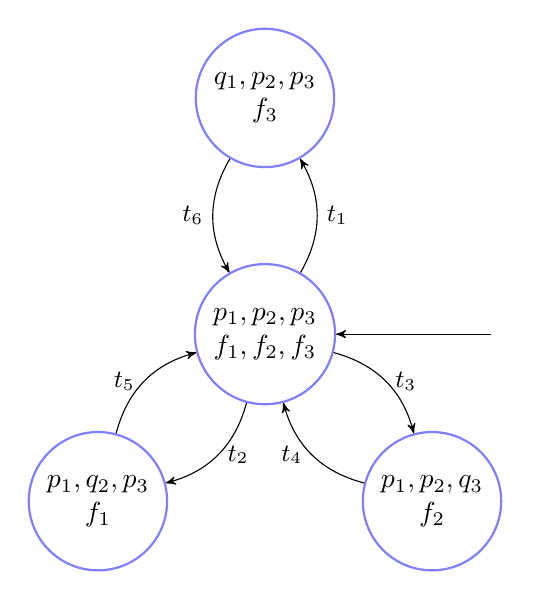
\begin{tikzpicture}[->, >=stealth', auto, node distance=3cm]
    \node[marking] (1)                    {$p_1, p_2, p_3$ \\ $f_1, f_2, f_3$};
    \node[marking] (2) [above of=1]       {$q_1, p_2, p_3$ \\ $f_3$};
    \node[marking] (3) [below left of=1]  {$p_1, q_2, p_3$ \\ $f_1$};
    \node[marking] (4) [below right of=1] {$p_1, p_2, q_3$ \\ $f_2$};
    \node (init) [right of=1] {};

    \path[every node/.style={font=\sffamily\small}]
      (init) edge (1)
      (1) edge[bend right] node [right] {$t_1$} (2)
      (2) edge[bend right] node [left] {$t_6$} (1)
      (1) edge[bend left] node [right] {$t_2$} (3)
      (3) edge[bend left] node [left] {$t_5$} (1)
      (1) edge[bend left] node [right] {$t_3$} (4)
      (4) edge[bend left] node [left] {$t_4$} (1);
  \end{tikzpicture}
  \caption{Une soirée chez Platon}
	\label{fig:marking}
\end{figure}

En admettant que la classe Swift suivante représente un noeud d'un graphe de marquage,
représentez le graphe de marquade de la figure \ref{fig:marking} en Swift:

\begin{lstlisting}[morekeywords={class,let,init,self}]
class MarkingGraph {
  let marking   : PTMarking
  let successors: [MarkingGraph]

  init(marking: PTMarking, successors: [MarkingGraph]) {
    self.marking    = marking
    self.successors = successors
  }
}
\end{lstlisting}

\end{document}
